\chapter{Problemstellung}
Immer wieder kommen Kunden der Senozon AG mit Fragestellungen wie \glqq{}Was passiert, wenn diese Strasse gesperrt wird?\grqq{} oder \glqq{}Was wäre, wenn  ein Neubaugebiet mit 5000 Einwohnern gebaut wird?\grqq{}. Bislang waren diese Fragestellungen mit viel Handarbeit verbunden, um das Modell anzupassen. Dies insbesondere, weil die Simulationsdaten von MATSim XML-basiert und meist sehr gross sind.\\
Derzeit kann lediglich die Senozon AG selbst die Änderungen an den Verkehrsmodellen vornehmen, weil dies nur mit dem erforderlichen Know-How und der entsprechenden Erfahrung möglich ist. Das Entwickeln einer Web Applikation soll diese Funktion zukünftig auch dem Kunden auf eine einfache Art und Weise zur Verfügung stellen. Dies würde die Arbeit der Senozon AG deutlich erleichtern, weil dann die Kunden selbst oder mit Unterstützung von Senozon AG ihre Daten für die Simulation aufbereiten können. Ziel dieser Arbeit ist es, die Konzepte und wesentlichsten Risiken einer solche Web Applikation, die das Bearbeiten eines Verkehrsmodells ermöglicht, zu analysieren. Zudem wurde ein Prototyp erstellt, der die erkannten Risiken beseitigt und die wichtigsten Konzepte umsetzt.
\section{Simulationsdaten}
Die Simulationssoftware MATSim arbeitet mit dateibasierten Simulationsdaten, d.h. alle benötigten Daten für die Simulation werden in XML Dateien zur Verfügung gestellt. Diese XML Dateien können bis zu mehreren Gigabytes gross werden, wenn es sich um grössere Netzwerke, wie z.B. das Netz der gesamten Schweiz oder Deutschland, handelt.\\
Das Verkehrsmodell-Netzwerk, welches der relevante Teil der Daten für unsere Arbeit darstellt, besteht aus mehreren Nodes und Links. Wie aus Abbildung \ref{example_street} ersichtlich ist, setzt sich eine Strasse aus zwei Nodes, welche die Endpunkte darstellen und einem Link, der die Verbindung zwischen diesen beiden Nodes aufzeigt.
\begin{figure}[H]
\centering
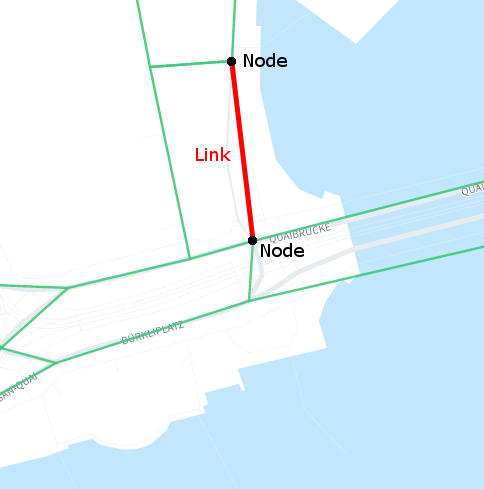
\includegraphics[height=7cm]{images/Link_demo_edited.PNG}
\caption{Beispiel Strasse: Nodes mit Link verbunden}
\label{example_street}
\end{figure}
\noindent
Ein Link stellt somit eine klassische Strasse aus dem Verkehrsnetz dar. Im Verkehrsmodell wird oft eine Strasse in mehrere Links unterteilt, da für jeden Abschnitt eigene Eigenschaften gelten. Wie in Abbilung \ref{street_details} ersichtlich, werden diese Eigenschaften zusammen mit den IDs der beiden Nodes des Links direkt auf dem Link gespeichert. Die genaue Position dieser Strasse erfahren wir somit durch die X und Y Koordinaten der beiden \glqq{}from\grqq{}- und \glqq{}to\grqq{}-Nodes.
\begin{figure}[H]
\centering
\lstset{language=XML}
\begin{lstlisting} [backgroundcolor = \color{white}]
<node id="1" x="680827" y="4825897"/>
<node id="2" x="680841" y="4825447"/>
<link id="3" 
	from="1" 
	to="2" 
	length="450" 
	freespeed="13.9" 
	capacity="1964.0" 
	permlanes="2.0" 
	oneway="1" 
	modes="car"
/>
\end{lstlisting}
\caption{XML Beispieldaten einer Strasse}
\label{street_details}
\end{figure}
\noindent
Für die Bearbeitung dieser Daten verwendet die Senozon AG zur Zeit eine Client Applikation, die direkt mit den XML Dateien arbeitet. Dies führt dazu, dass diese Applikation sehr arbeitsspeicherintensiv ist, um trotzdem performant zu sein. Daher ist diese Applikation nicht für den Einsatz beim Kunden vor Ort geeignet.
\section{Änderungsmanagement}
Die bisherigen Änderungen an einem Verkehrsmodell wurden direkt an den vorhandenen Stammdaten vorgenommen. Dies führt dazu, dass die Stammdaten redundant in verschiedenen Verkehrsmodellen vorhanden sind. Dadurch müssen bei Änderungen der Stammdaten immer wieder alle Verkehrsmodelle überarbeitet werden.\\
In der Web Applikation sollen alle Benutzer mit denselben Stammdaten arbeiten können und nur die Änderungen individuell abgespeichert werden. Dadurch wird der benötigte Speicherplatz deutlich verringert und auch die Änderung der Stammdaten stellt somit kein Problem mehr dar.\\